\chapter{Windows 10のモダンマネージメントの概要}
\label{chap:モダンマネージメント}

\section{Windows 端末の利用形態}

Windows 端末では、何でもできてしまうのが利点ですが、何でもできるようにしてしまうと設定費用が増えてしまうとともに、日々の運用負担も増えてしまいます。ここでは、まずWindowsデバイスの利用形態について考えてみたいと思います。

Microsoft GIGAスクールパッケージでは、3種類の利用方法を想定しています(参照:図\ref{fig:Windowデバイスの利用形態1})。それぞれの端末に関して説明していきます。

\begin{description}
    \item[キオスク端末]\mbox{}\\
    Windows 10 には「割り当てられたアクセス(Assigned Access)」という機能が備わっており、ストアアプリを1つだけ実行できる特殊なアカウントを作成できる「キオスクモード(Kiosk Mode)」というものがあります。公共施設に設置されている検索専門端末、店頭のデモPC、デジタルサイネージ(電子看板、デジタル広告)などに利用されています。キオスク端末では電源を入れると、指定されたアプリ(Webブラウザなど)が立ち上がりログインすることなく、すぐに利用することが可能です。
    \item[共有端末(おすすめ)] \mbox{}\\
    共有端末は1台の端末を複数のユーザーがログインして利用することができる端末です。Windows 10 PC の「共有PCモード」を有効にすることで利用できるようになります。共有端末はActive Directory または Azure Active Directory に参加させることができ、これによりディレクトリー内の全てのユーザーがログインできるようになります。共有PCモードでアカウント管理サービスをオンにすると、アカウントは自動的に削除されます。アカウント管理は、サインオフ時とシステムメンテナンス時の両方で実行され、サインアウト直後またはディスク領域が少ない場合にアカウントを削除するように構成できます。Windows 10 Version 1703 以降では、サインインしない状態が指定日数を超えた場合にアカウントを削除する非アクティブオプションが追加されました。

    共有 PC モードは、PC を使用していない時間を活用してメンテナンスを行うよう設定されています。従って、メンテナンスの実行、アカウントのクリーンアップ、Windows Update の実行時にPCがスリープ状態を解除できるようにしておく必要があります。共有PCモードでは、Windows Update 自体の構成はできませんが、Intune を使って、メンテナンス時間中にWindows Upateを行い、必要に応じて再起動するように設定することができます。これにより Windows PC は常に最新の状態を保つことができ、授業中に更新プログラが適用され授業ができないといったことを防ぐことができます。
    \item[1 to 1端末(BYOD端末)] \mbox{}\\
    1 to 1 端末は、1人の特定のユーザーしかログインして利用しない端末で、教職員が利用する端末やBYOD(Bring Your Own Device/自分のデバイスを持ち込む)がこれに該当します。1 to 1 端末では、Microsoft アカウント\footnote{Microsoft アカウントとはWindowsやXbox Live、outlook.comなどのクラウドクラウサービスにサインインするためのアカウントです。}やローカルアカウントで、Windows にログインしている状態で学校のアカウント\footnote{ここでは、Azure Active Directory のアカウントをさします。}で利用できるサービス(Office 365 ProPlusやOneDrive for Businessなど)も利用できるようにできます。
\end{description}

GIGAスクール構想で児童・生徒が利用する端末は、運用・メンテナンスの省力化を行うため\textbf{共有端末(共有PCモード)}で提供することを強くお勧めします。


\begin{figure}[htbp]
    \centering
    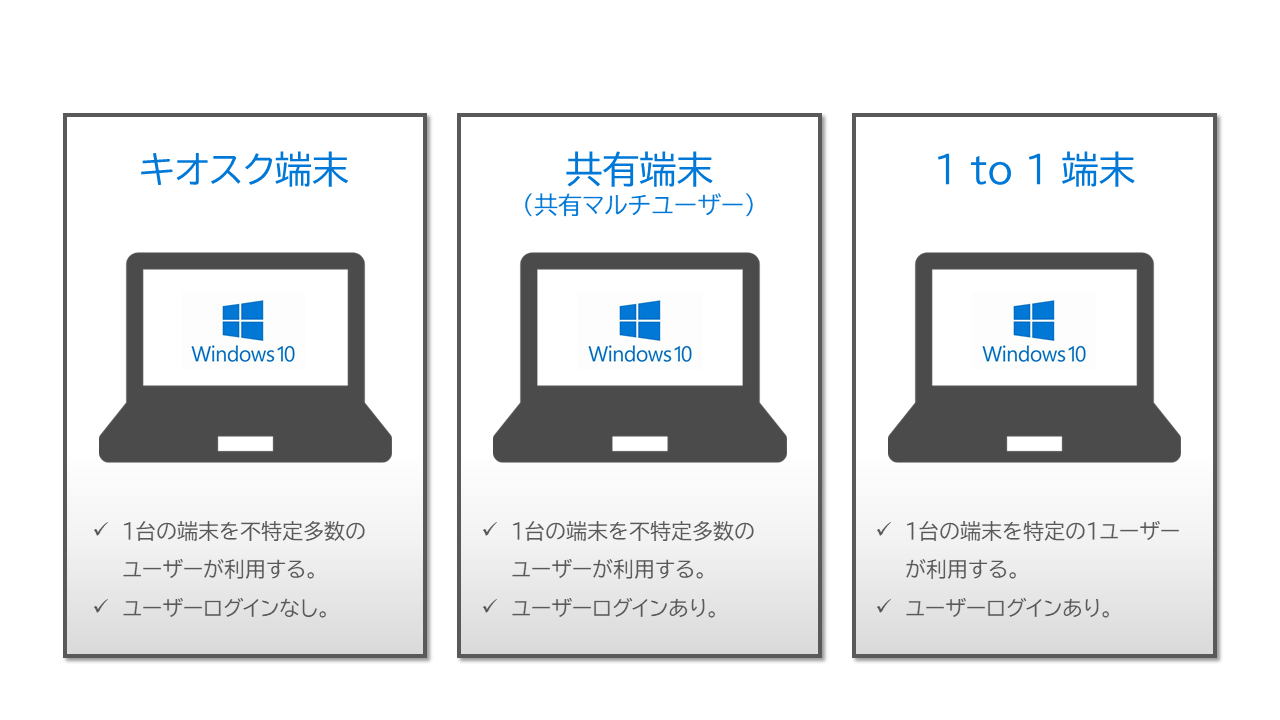
\includegraphics[width=12cm]{figures/HowtoUsePC-1.png}
    \caption{Windows デバイスの利用形態1}
    \label{fig:Windowデバイスの利用形態1}
\end{figure}

次にデバイス上でどのようなアプリケーションを利用していくかについて考えてみましょう。ここでもマイクロソフトでは3種類のモデルを想定しています。

\begin{description}
    \item[ライトモデル]\mbox{}\\
    ライトモデルは、Webブラウザ(Microsoft Edge)のみが利用できるモデルです。
    \item[ミドルモデル]\mbox{}\\
    ミドルモデルは、Webブラウザ、Office 365 ProPlus(Word、Excel、PowerPoint、Teamsなど)とMicrosoftストアーで提供されるアプリ(ホワイドボードやMinecraftなど)が利用できるもです。
    \item[フルモデル]\mbox{}\\
    フルモデルは、ミドルモデルにインストールされているアプリ以外にも授業等で利用するアプリケーションがインストールされているモデルになります。
\end{description}

ライトモデルとミドルモデルは、Microsoft GIGAパッケージで推奨するディプロ方法(Provisioning Package と Intune for Education)でディプロイすることが可能です。フルモデルに関しては、Intune for Education でインストールできるアプリケーションとインストールできないアプリケーションがありますので注意してください。

\begin{figure}[htbp]
    \centering
    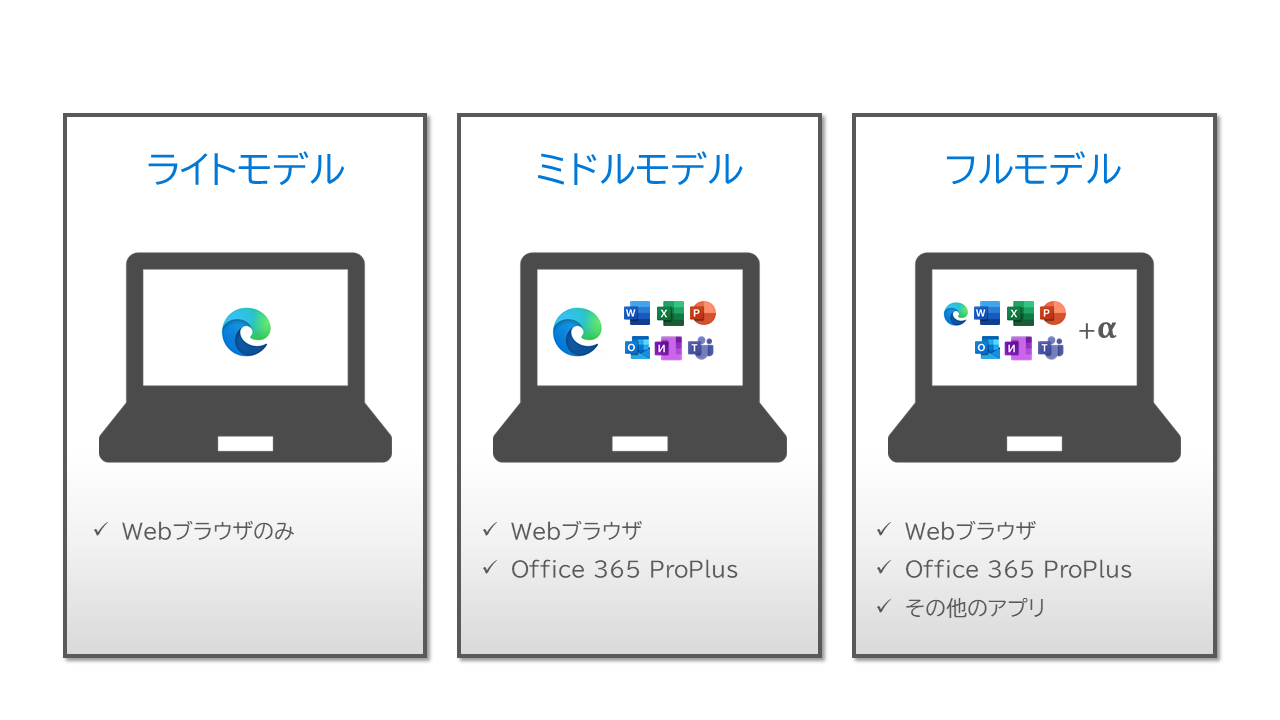
\includegraphics[width=12cm]{figures/HowtoUsePC-2.png}
    \caption{Windows デバイスの利用形態2}
    \label{fig:Windowデバイスの利用形態2}
\end{figure}

\section{マスターテンプレート方式(従来型)とモダンマネージメントによるディプロイ方式}

Window 7や8のディプロイをやったことのある方々にはなじみの方法だと思いますが、これまでは1台のPCをセッティングして、そのPCからマスターイメージを作成し
、そのマスターイメージを使用してクローニングすることで、大量のPCを一度にキッティングしていました。この方法は、物理コピーだけなので作業効率が高く、品質も均一化することができます。PCを並べる場所と電源に余裕があれば、数百台でも短期間で量産することが可能です。


\begin{figure}[htbp]
    \centering
    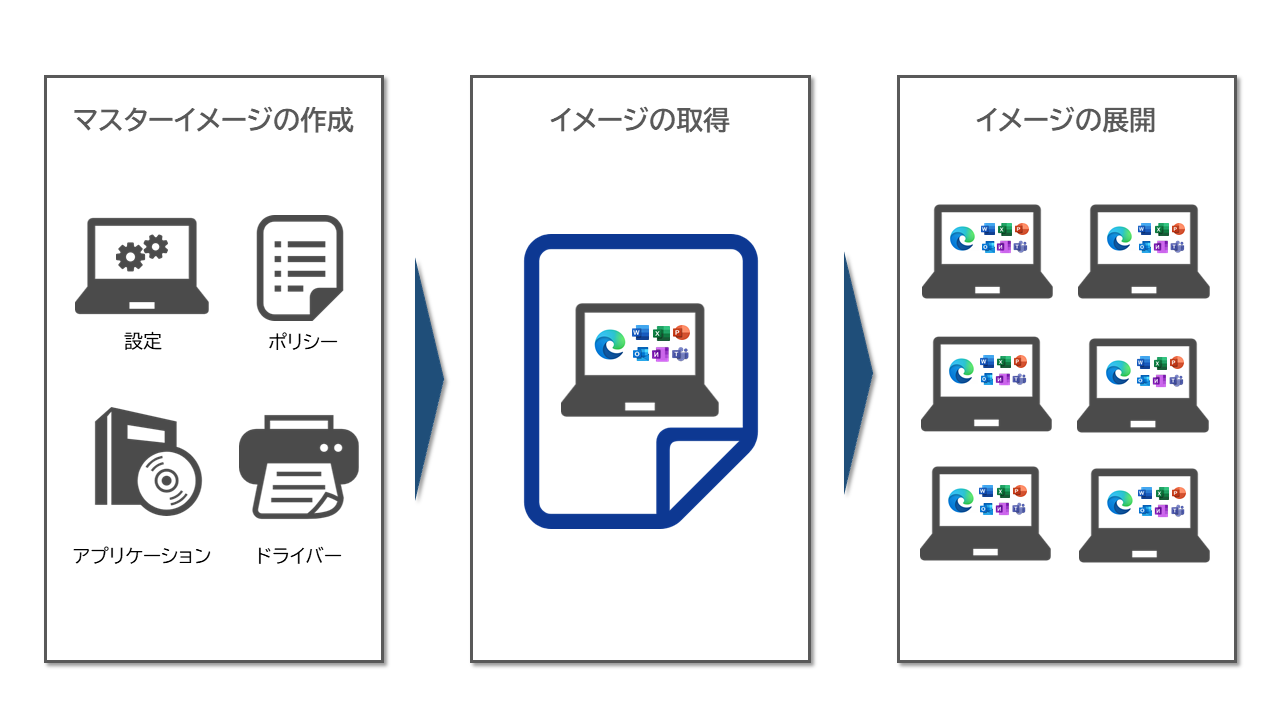
\includegraphics[width=12cm]{figures/MasterImage.png}
    \caption{マスターイメージを使った展開方法}
    \label{fig:MasterImage}
\end{figure}

それに対して、Provisioning Package もしくは Autopilot と Intune を使った方法をここでは「\textbf{Windows 10 のモダンディプロイ}」と呼びます。もちろん従来型のマスターイメージを使った展開方法で Windows 10 はディプロイできないわけではありません。しかし、マスターイメージを作成するのに数週間から1ヶ月かかるマスターイメージを使った展開方法は、Windows 10 のディプロイには向いていません。では、なぜ向いていないのか\ref{sec:WaaS}項で解説したいと思います。

\section{Windows as a Service (WaaS)とは何か?}
\label{sec:WaaS}

まず、「WaaS」とは何かについて説明していきます。従来の Windows OS では、Windows 7 から Windows 8 などのような「\textbf{メジャーバージョン}」に加えて、「\textbf{サービスパック}」として新たな機能が追加されてきました。Windows 7 SP1 の「SP1」がまさにそのサービスパックに該当します。

Windows OS を利用していく上で常に最新の「サービスパック」を適応していくことが望ましいですが、従来はある程度時間的な執行猶予が存在していました。例えば Windows 7 SP1 が提供開始されたのは、2011年2月ですが、Windows 7 のサポート終了は2013年4月でした。つまり、SP1の適用には2年程度の猶予が会ったことになります。

一方 Windows 10 では、従来の「サービスパック」に相当する「\textbf{機能更新プログラム}」が年2回提供されています。これにより Windows 10 にはバージョンアップという概念がなくなり、半年ごとに新たな機能が加わっていくことになります。

ここで重要なのが、それぞれの「更新プログラム」が適用された状態のサポート期間は18ヶ月となっている点です。そのため、継続的にサポートを受けた目には、新たな機能が不要だとしても「機能更新プログラム」の適用を続けていく必要があります。

つまり、「\textbf{モノ+サポート}」という考え方ではなく、常に新たな機能を提供する「\textbf{サービス}」としてOSを捉えているわけだ。こうした新たなWindows OSの在り方が
「\textbf{WaaS(Windows as a Service)}」(=サービスとしてのWindows)なのです。

\begin{figure*}[htbp]
    \centering
    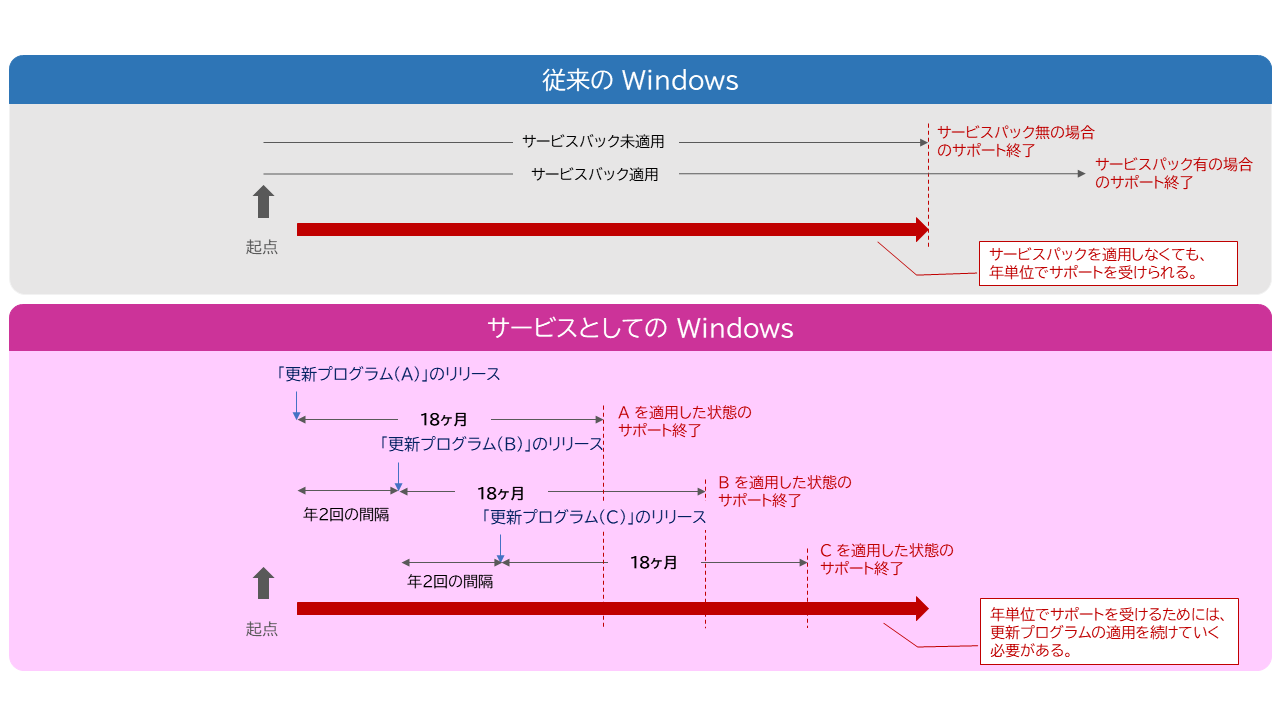
\includegraphics[width=17cm]{figures/WaaS.png}
    \caption{従来のWindowsとWindows 10のライフサイクルの違い}
    \label{}
\end{figure*}

上記に述べた「Windows 10 の年2回の機能更新、それぞれのサポートが18ヶ月間」という形態は「\textbf{Semi-Annual Channel(SAC)}」、日本語表記は「\textbf{半期チャネル」}と呼ばれています。Windows 10 では、組み込み機器など「機能更新プログラム」の適用が難しい特殊な用途向けには数年間単位で現状のOS状態が維持できる「\textbf{Long-Term Servicing Channel (LTSC)}」という形態も用意されておりますが、いくつか制約条件もあるため、GIGAスクール構想のPCではSACを利用することを強く推奨します。

従って、Windows 10 を利用していく上では、年2回の頻度で機能更新プログラムを適用していく必要があります。

\section{Windows 10 へ移行すると運用管理が変わる}
\label{sec:Win10の運用}

\ref{sec:WaaS}項でも説明したように、Windows 10 には WaaSという概念があって、継続的なバージョンアップによって新しい機能やデザインが都度追加されていきます。これは従来のWindows管理手法から、その方法が大きく変わることを意味しています。

Microsoft GIGAスクールパッケージ対応PCに搭載されている Windows 10 Pro Education では、「\textbf{Windows Update for Business}」というアップデート機能が備わっています。Active Directory や Azure Active Directory のグループポリシーや、Intune のポリシーに沿って、アップデートのタイミングなどをコントロールできるため、従来のWindows に比べて計画的なアップデート作業全般を一元化することができます。これにより夜間ユーザーが利用していないときに Windows OS のアップデートを行うことができるわけです。

GIGAスクール構想では、令和2年度から令和5年度までの4年間に渡りデバイスの調達が行われます。従って翌年度同機種のデバイスが購入できるとは限りません。Windows 10 は年に2回バージョンアップがありますので、マスターイメージ方式では半年ごとにすべての保有する機種のイメージを再作成する必要が出てきます。従ってマスターイメージを使った運用方法では、年を追うごとに作業量が増えていくわけです。

\begin{figure}[htbp]
    \centering
    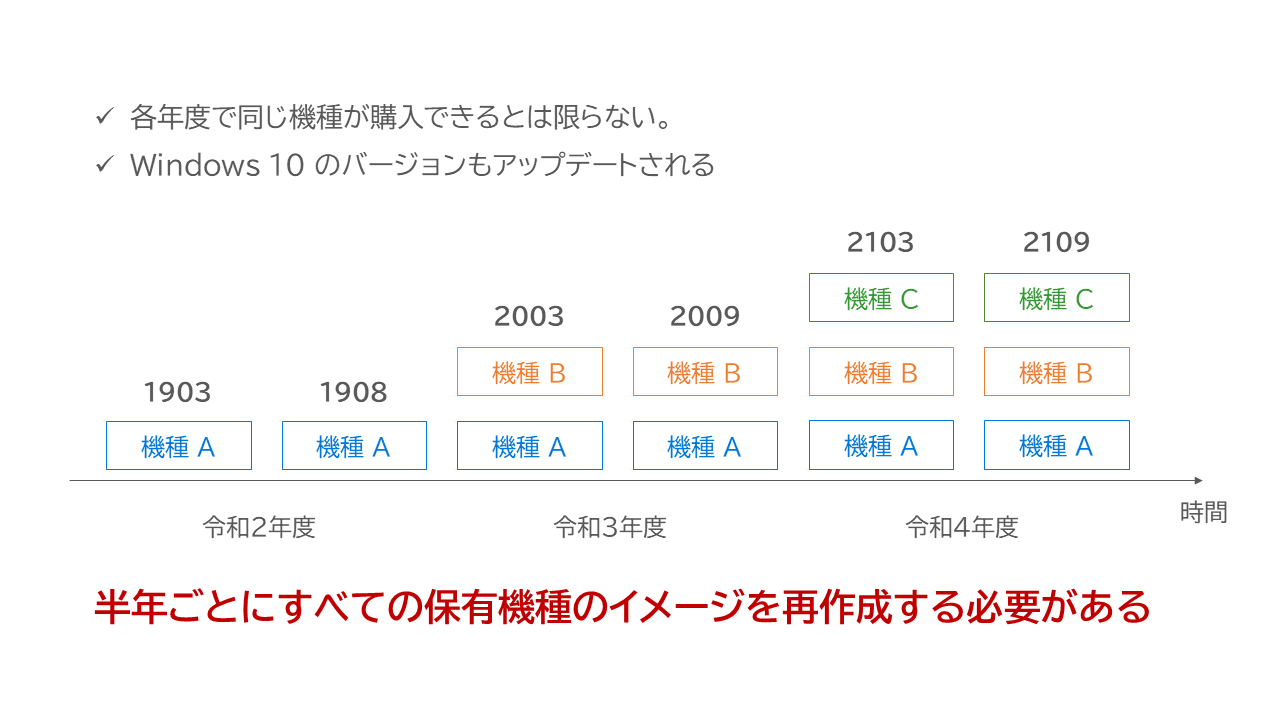
\includegraphics[width=14cm]{figures/MasterImage2.png}
    \caption{マスターイメージ方式の課題}
    \label{fig:MasterImage2}
\end{figure}

このためWindows 10 にあった運用方法であるモダンマネージメントが必要なのです。\ref{sec:ProvisioningPackage1}項では、マイクロソフトが提唱するWindows 10 のモダンマネージメントである「Provisioning Package」と「Autopilot」についての違いについて解説致します。


\section{Provisioning Package と Autopilot}
\label{sec:ProvisioningPackage1}

Windows PC を購入して、はじめて電源を入れたとき、図\ref{fig:Win10_Kitting}のような画面が表示されて、1画面づつマウスやキーボードを使い設定していきます。「Provisioning Package」と「Autopilot」はどちらもほぼ同じようなことをやっています。言語やキーボードなどの初期設定から、Active Directory や Azure Active Directory にデバイスを参加させ、そのデバイスを モバイルデバイス管理(MDM)に登録します。

違いは何かというと「Provisioning Package」は、Windows 構成デザイナーというツールを使って図\ref{fig:Win10_Kitting}で手作業でやっている作業を自動化することができます。一方 AutoPilot はネットワーク越しに、組織のポリシーを設定していきますので、インターネットに接続できるところまでは作業が済んでていることが前提となりますのでBYOD端末の設定に向いているディプロイ方法です。

GIGAスクール構想のように学校自身が一括でデバイスを調達し、それを児童・生徒に配布する場合には、「Provisioning Package」を使ったディプロイの方が向いています。「Provisioning Package」使ったディプロイ方法に関して、第\ref{cap:Win10_deploy}章で解説いたします。

\begin{figure*}[t]
    \centering
    \vspace{-6cm}
    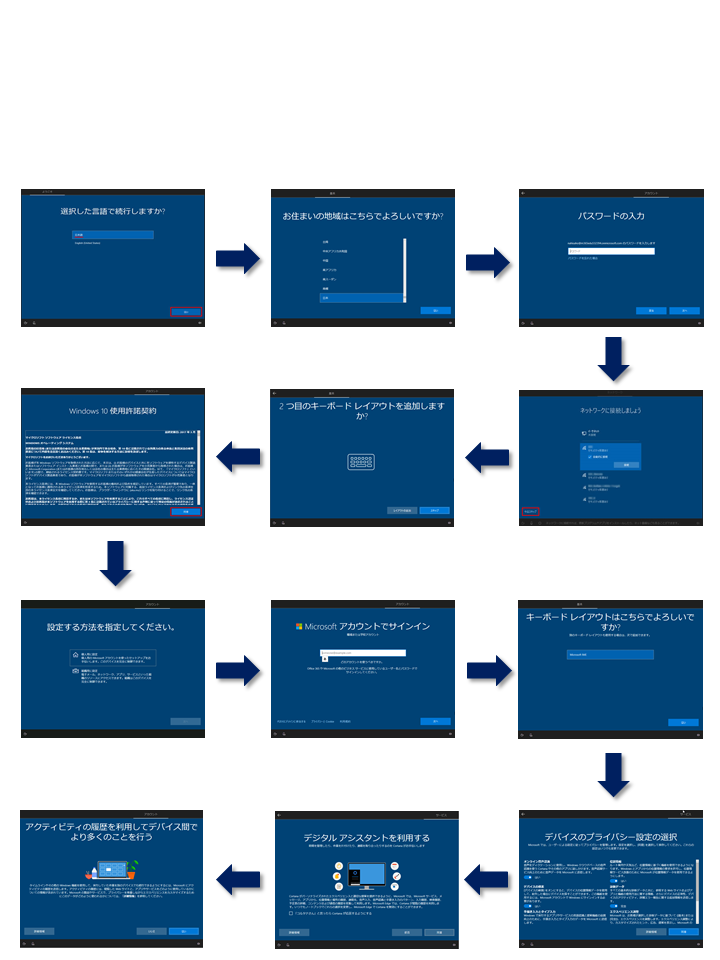
\includegraphics[width=17cm]{figures/Win10_Kitting.png}
    \caption{Windows 10 の初期設定のフロー}
    \label{fig:Win10_Kitting}
\end{figure*}


\chapter{Windows端末の展開手順の概要}
\label{chap:Windows端末の展開手順の概要}

第\ref{chap:Windows端末の展開手順の概要}章ではWindowsデバイスのモダンディプロイ作業における作業手順の概要に関して解説していきます。図\ref{fig:StepbyStep}は、Windows 端末展開手順を示したものです。以下に各作業の説明をします。

\begin{figure*}[htbp]
    \centering
    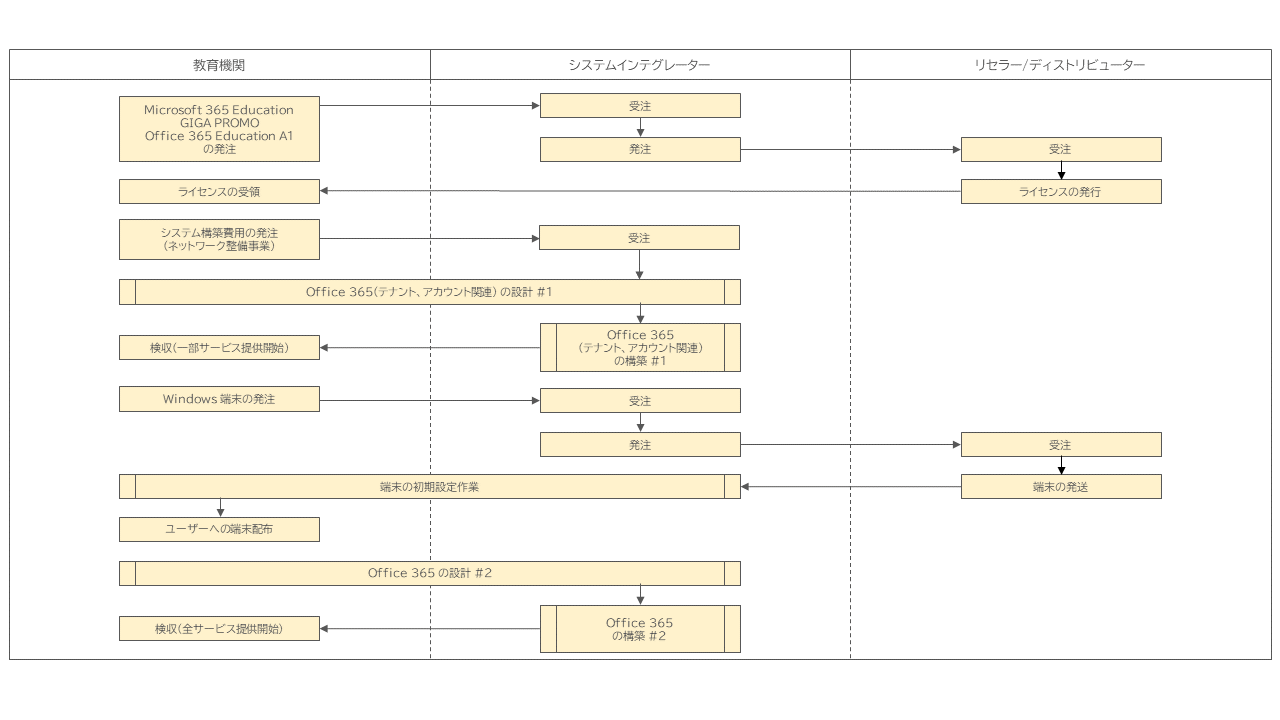
\includegraphics[width=17cm]{figures/StepbyStep.png}
    \caption{Windows 端末の展開手順}
    \label{fig:StepbyStep}
    \vspace{15cm}
\end{figure*}

\begin{description}
    \item[ライセンスの発注]\mbox{}\\
    教育機関は、Microsoft 365 GIGA PROMO と Office 365 A1 ライセンスの発注を行ってください。Microsoft 365 GIGA PROMO は、モバイルデバイス管理(MDM)ですので、端末整備事業に該当しします。
    \item[Office 365のアカウント管理、初期設定作業の発注]\mbox{}\\
    Windows モダンディディプロイを行うためには、Office 365 のアカウント管理、認証基盤である Azure Active Directory にアカウントの登録をするとともに、デバイス管理に必要な Office 365 の設定を行う必要がございます。こちらはネットワーク整備事業に該当します。
    \item[Office 365の設定 その1]\mbox{}\\
    Windows デバイスのモダンディプロイを行うための最低限の設定を行います。ここで行う作業は、
        \begin{enumerate}
            \item Office 365 A1 のテナントの取得
            \item Office 365 のカスタムドメインの作成
            \item Office 365 へのアカウントの登録
        \end{enumerate}
    です。
    \item[Provisioing Package の作成]\mbox{}\\
    Windows 構成デザイナーを使って Provisionig Package を作成します。
    \item[Provisioing Package を使った端末のディプロイ] \mbox{}\\
    Provisioing Package を使って Windows 端末の初期設定を行います。
    \item[Intune for Education による端末管理] \mbox{}\\
    端末管理サービス(MDM)の Intune for Education を使用してWindows端末を管理します。
    \item[Office 365の設定 その2] \mbox{}\\
    Office 365 を安全・安心してお使いいただくための、設定を行います。
    
\end{description}
